\chapter{СОСТАВЛЕНИЕ МАТЕМАТИЧЕСКОЙ МОДЕЛИ ПНЕВМОПРИВОДА}\label{ch:ch2}
Данная глава посвящена математическому моделированию ПП
с дискретными распределителями. Рассматриваются следующие ключевые аспекты:

\begin{enumerate}
    \item Структура и принцип работы исследуемого ПП;
    \item Моделирование пневмоцилиндра;
    \item Моделирование дискретных распределителей;
    \item Моделирование силы трения и упругих деформаций;
    \item Адаптация математической модели к эффективному численному расчету на ЭВМ.
    \item Верификация математической модели.
\end{enumerate}

Математическая модель включает:

\begin{enumerate}
    \item Уравнения движения поршня;
    \item Уравнения изменения давления в полостях цилиндра;
    \item Уравнения изменения температуры рабочего тела в полостях цилиндра;
    \item Модель массового расхода воздуха;
    \item Модель динамики распределителей;
    \item Модель сил трения;
    \item Модель силы реакции опоры.
\end{enumerate}

Используются уравнения термодинамики и газовой динамики. Учитываются нелинейные эффекты:
сжимаемость воздуха, особенности течения через дросселирующие элементы, силы трения и реакции опоры.

Верификация модели проводится путем проверки математической корректности.


\section{Структура и принцип работы исследуемого пневмопривода}\label{sec:ch2/sec1}
Исследуемый электропневматический привод включает пневматический цилиндр двустороннего действия
c односторонним штоком и четыре двухпозиционных распределителя.
Цилиндр содержит две рабочие полости, разделенные поршнем.

Ключевой особенностью привода является конфигурация распределителей.
К каждой полости цилиндра подключены два независимых распределителя:
один для подачи сжатого воздуха из магистрали, другой для выхлопа в атмосферу.
Такая конфигурация обеспечивает гибкое управление потоками воздуха в обеих полостях цилиндра.

\begin{figure}[h]
    \centerfloat{
        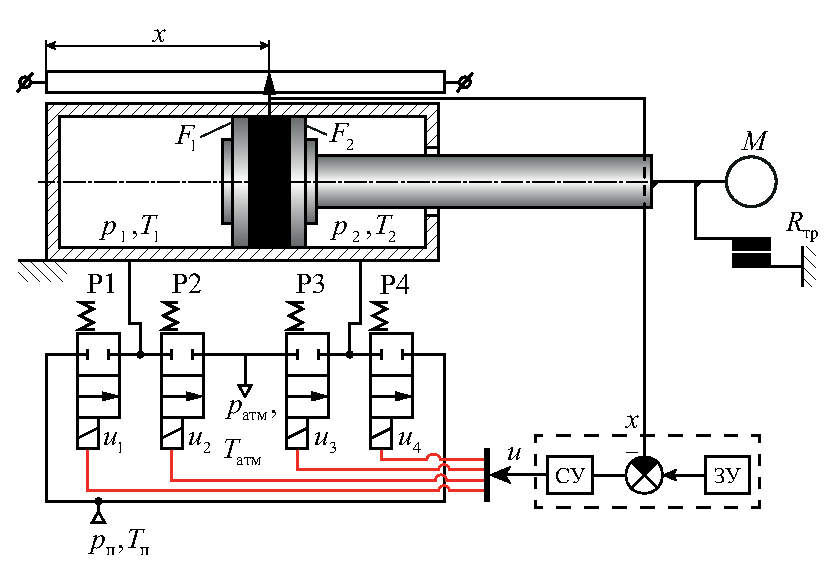
\includegraphics[]{part2/расчетная_схема_привода.eps}
    }
    \caption{Принципиальная пневматическая схема исследуемого привода}
    \label{fig:ch2/pneumatic_actuator_scheme}
    
\end{figure}

Каждый распределитель имеет два дискретных состояния: открыто и закрыто.
Общее количество возможных комбинаций состояний распределителей
определяется формулой:
\begin{equation}
    N = 2^k,
\end{equation}
где $N$ - число комбинаций, $k$ - количество распределителей.

Для рассматриваемой системы с четырьмя распределителями:
\begin{equation}
    N = 2^4 = 16.
\end{equation}

Таким образом, система имеет 16 дискретных состояний, что обеспечивает широкие возможности
управления при сохранении относительной простоты конструкции.

Система управления генерирует дискретные сигналы для активации
электромагнитных клапанов распределителей. Обратная связь по положению реализуется посредством датчика линейного перемещения на штоке цилиндра. 

Использование дискретных распределителей вместо пропорциональных, как было сказано ранее,
снижает стоимость системы, однако требует разработки более сложных
алгоритмов управления для компенсации нелинейного характера коммутации пневматических линий.

\section{Моделирование пневмоцилиндра}\label{sec:ch2/sec2}

При разработке математической модели пневмоцилиндра были приняты следующие основные допущения:
\begin{enumerate}
    \item Рабочим телом является идеальный газ (воздух), подчиняющийся уравнению состояния Клапейрона-Менделеева;
    \item Процессы в рабочих полостях пневмоцилиндра рассматриваются как адиабатические, теплообмен с окружающей средой не учитывается;
    \item Температура газа в магистрали и температура окружающей среды принимаются постоянными;
    \item Утечки газа через уплотнения поршня и штока не учитываются;
    \item Давление в выхлопной магистрали принимается равным атмосферному;
    \item Влияние сил тяжести на движение поршня не учитывается ввиду горизонтального расположения пневмоцилиндра;
    \item Пневматические линии между распределителями и рабочими полостями цилиндра считаются короткими,
          их объем пренебрежимо мал по сравнению с объемом рабочих полостей;
    \item Эффекты сжимаемости воздуха в трубопроводах не учитываются.
\end{enumerate}

С учетом принятых допущений, математическая модель пневмоцилиндра может быть представлена системой
дифференциальных уравнений, описывающих изменение давлений в рабочих полостях, температур газа и
движение поршня. Данная система уравнений формирует основу для дальнейшего анализа динамики пневмопривода
и синтеза алгоритмов управления.

\subsection{Уравнение движения пневмоцилиндра}\label{sec:ch2/sec2/subsec1}

Рассмотрим пневмоцилиндр как систему с одной степень свободы. Обобщенной координатой выберем положение поршня $x$.
Для применения принципа Гамильтона необходимо составить функцию Лагранжа:
\begin{equation}
\label{eq:ch2/eq0}
    L = T - U,
\end{equation}
где $T$ -- кинетическая энергия системы; $U$ -- потенциальная энергия системы; $L$ -- функция Лагранжа.

Кинетическую энергию системы можно представить в виде:
\begin{equation}
\label{eq:ch2/eq1}
    T = \frac{M}{2} \dot{x}^2,
\end{equation}
где $M$ -- масса подвижных частей системы; $\dot{x}$ -- скорость движения поршня.

Потенциальная энергия системы включает в себя работу силы давления газа в рабочих полостях цилиндра:

\begin{equation}
\label{eq:ch2/eq2}
    U = p_1 V_1 + p_2 V_2 + p_\text{атм} (V_1 - V_2),
\end{equation}
где $p_1$ и $p_2$ -- давления в рабочих полостях цилиндра;
$V_1$ и $V_2$ -- объемы рабочих полостей;
$p_\text{атм}$ -- атмосферное давление.

Объемы рабочих полостей связаны с положением поршня следующим образом:
\begin{equation}
\label{eq:ch2/eq3}
    \begin{aligned}
        V_1 & = F_1 (x - x_0),     \\
        V_2 & = F_2 (L - x + x_0),
    \end{aligned}
\end{equation}
где $F_1=\pi D_{поршня}^2/4 $ и $F_2 = \pi (D_{поршня}^2/4 - D_{штока}^2/4)$ -- активные площади поперечного сечения поршня в поршневой и штоковой полостях соответственно;
$x_0$ -- начальное положение поршня;
$L$ -- ход поршня.

Подставляя \eqref{eq:ch2/eq1}, \eqref{eq:ch2/eq2} и \eqref{eq:ch2/eq3} в \eqref{eq:ch2/eq0}, получим функцию Лагранжа:

\begin{equation}
\label{eq:ch2/eq4}
    \begin{aligned}
        L & = \frac{M}{2} \dot{x}^2 - p_1 F_1 (x - x_0) - p_2 F_2 (L - x + x_0) \\
          & - p_\text{атм} (F_1 (x - x_0) - F_2 (L - x + x_0)).
    \end{aligned}
\end{equation}

Обобщенную силу $Q_x$, действующую на систему учитывающую силу трения и реакции упоров, можно представить в виде:
\begin{equation}
\label{eq:ch2/eq5}
    Q_x = - R_{\text{тр}} - R_{\text{упор}},
\end{equation}
где $R_{\text{тр}}$ -- сила трения; $R_{\text{упор}}$ -- сила реакции упора.

Запишем уравнение лагранжа в общем виде:

\begin{equation}
\label{eq:ch2/eq6}
    \frac{d}{dt} \left( \frac{\partial L}{\partial \dot{x}} \right) - \frac{\partial L}{\partial x} = Q_x.
\end{equation}

Вычислим частные производные функции Лагранжа \eqref{eq:ch2/eq4} по обобщенной координате $x$ и ее производной $\dot{x}$:

\begin{equation}
\label{eq:ch2/eq7}
    \begin{aligned}
        \frac{\partial L}{\partial \dot{x}} & = M \dot{x},                                    \\
        \frac{\partial L}{\partial x}       & = p_1 F_1 - p_2 F_2 - p_\text{атм} (F_1 - F_2).
    \end{aligned}
\end{equation}

Подставляя \eqref{eq:ch2/eq7} и \eqref{eq:ch2/eq5} в \eqref{eq:ch2/eq6}, получим уравнение движения пневмоцилиндра:

\begin{equation}
\label{eq:ch2/eq8}
    M \ddot{x} = p_1 F_1 - p_2 F_2 - p_\text{атм} (F_1 - F_2) - R_{\text{тр}} - R_{\text{упор}}.
\end{equation}
где $\ddot{x}$ -- ускорение поршня.

\subsection{Уравнения изменения давлений в полостях пневмоцилиндра}\label{sec:ch2/sec2/subsec2}

Первоначально получим дифференциальные уравнения изменения давлений в
полостях пневмоцилиндра, основываясь на началах термодинамики
и уравнения Максвелла с учетом ранее принятых допущений.
Ключевыми допущениями для данного вывода являются: рассмотрение
воздуха как идеального газа, адиабатический характер процессов в полостях
цилиндра, отсутствие утечек газа через уплотнения, и пренебрежение объемом
пневматических линий между распределителями и рабочими полостями.

Согласно первому началу термодинамики для открытой системы, изменение внутренней энергии рабочего тела описывается уравнением:

\begin{equation}
\label{eq:ch2/first_law}
    dU = \partial Q - \partial W + hdm,
\end{equation}

где $dU$ - изменение внутренней энергии;
$\partial Q$ -- подведенное тепло;
$\partial W$ -- совершенная работа;
$h$ -- удельная энтальпия;
$dm$ -- изменение массы системы.

Учитывая, что процесс рассматривается как адиабатический,
то $\partial Q = 0$ и работа совершается только за счет изменения объема газа в полостях цилиндра:
\begin{equation}
\label{eq:ch2/work}
    \partial W = -pdV.
\end{equation}

Тогда уравнение изменения внутренней энергии примет вид:
\begin{equation}
\label{eq:ch2/internal_energy_change}
    dU = -pdV + hdm.
\end{equation}

Используя определение энтальпии $H - U = pV$, получим:
\begin{equation}
\label{eq:ch2/enthalpy_definition}
    d(H-pV) = -pdV + hdm.
\end{equation}

Раскрывая дифференциалы, получим:
\begin{equation}
\label{eq:ch2/enthalpy_differential}
    dH - pdV - Vdp = -pdV + hdm.
\end{equation}

Сокращая слагаемые, получим уравнение изменения энтальпии:
\begin{equation}
\label{eq:ch2/enthalpy_change}
    dH = Vdp + hdm.
\end{equation}

Обратимся к соотношению Максвелла для энтальпии, которое связывает изменение
энтальпии с изменением давления и температуры:
\begin{equation}
\label{eq:ch2/maxwell_enthalpy}
    dH = \left(
    \frac{\partial H}{\partial p}
    \right)_T dp + \left(
    \frac{\partial H}{\partial T}
    \right)_p dT.
\end{equation}

Приравнивая правые части уравнений \eqref{eq:ch2/enthalpy_change} и \eqref{eq:ch2/maxwell_enthalpy}, получаем:

\begin{equation}
\label{eq:ch2/enthalpy_equality}
    \left(
    \frac{\partial H}{\partial p}
    \right)_T dp + \left(
    \frac{\partial H}{\partial T}
    \right)_p dT = Vdp + hdm.
\end{equation}

Воспользуемся одним из соотношений Максвелла:
\begin{equation}
\label{eq:ch2/maxwell_relation}
    \left(
    \frac{\partial H}{\partial p}
    \right)_T = V - T \left(
    \frac{\partial V}{\partial T}
    \right)_p.
\end{equation}

Подставляя это выражение в \eqref{eq:ch2/enthalpy_equality}, получим:
\begin{equation}
\label{eq:ch2/enthalpy_substitution}
    \left( V - T \left(
        \frac{\partial V}{\partial T}
        \right)_p \right) dp + \left(
    \frac{\partial H}{\partial T}
    \right)_p dT = Vdp + hdm.
\end{equation}

После упрощения и группировки членов, приходим к следующему выражению:
\begin{equation}
\label{eq:ch2/enthalpy_simplified}
    -T \left(
    \frac{\partial V}{\partial T}
    \right)_p dp + \left(
    \frac{\partial H}{\partial T}
    \right)_p dT = hdm.
\end{equation}

Используем еще одно важное термодинамическое соотношение:
\begin{equation}
\label{eq:ch2/specific_heat}
    \left(
    \frac{\partial H}{\partial T}
    \right)_p = c_p,
\end{equation}
где $c_p$ -- удельная теплоемкость при постоянном давлении.

Подставляя \eqref{eq:ch2/specific_heat} в уравнение \eqref{eq:ch2/enthalpy_simplified}, получим:
\begin{equation}
\label{eq:ch2/enthalpy_final}
    -T \left(
    \frac{\partial V}{\partial T}
    \right)_p dp + c_p dT = hdm.
\end{equation}

Для идеального газа справедливо соотношение:
\begin{equation}
\label{eq:ch2/ideal_gas_relation}
    \left(\frac{\partial V}{\partial T}\right)_p = \frac{R}{p},
\end{equation}
где $R$ -- газовая постоянная.

Используя данное выражение, преобразуем уравнение:
\begin{equation}
\label{eq:ch2/pressure_temp_relation}
    -\frac{RT}{p} dp + c_p dT = h dm.
\end{equation}

Разделив обе части на $dt$ и учитывая, что $dm/dt = G$ (массовый расход), получаем дифференциальное уравнение:
\begin{equation}
\label{eq:ch2/differential_equation}
    -\frac{RT}{p} \frac{dp}{dt} + c_p \frac{dT}{dt} = hG.
\end{equation}

Теперь обратимся к уравнению состояния идеального газа:
\begin{equation}
\label{eq:ch2/ideal_gas_equation}
    pV = mRT.
\end{equation}

Дифференцируя его по времени, получаем:
\begin{equation}
\label{eq:ch2/ideal_gas_differential}
    V\frac{dp}{dt} + p\frac{dV}{dt} = RT\frac{dm}{dt} + mR\frac{dT}{dt}.
\end{equation}

Подставляя выражение для $dT/dt$ из уравнения \eqref{eq:ch2/differential_equation} и учитывая, что для идеального газа
\begin{equation}
\label{eq:ch2/specific_heat_difference}
    c_p - c_v = R,
\end{equation}
где $c_v$ -- удельная теплоемкость при постоянном объеме, после ряда алгебраических преобразований получаем:
\begin{equation}
\label{eq:ch2/pressure_change}
    \frac{dp}{dt} = \frac{\gamma}{V}\left(RT\frac{dm}{dt} - p\frac{dV}{dt}\right),
\end{equation}
где $\gamma = c_p/c_v$ -- показатель адиабаты.

Учитывая, что к каждой полости пневмоцилиндра подключены два независимых распределителя:
один для подачи сжатого воздуха из магистрали, другой для выхлопа в атмосферу,
запишем уравнение \eqref{eq:ch2/pressure_change} для обеих полостей:

\begin{equation}
\label{eq:ch2/pressure_system}
    \begin{cases}
        \begin{aligned}
            \frac{dp_1}{dt} & = \frac{\gamma}{V_1}\left(RT_1\frac{dm_1}{dt} - p_1\frac{dV_1}{dt}\right), \\
            \frac{dp_2}{dt} & = \frac{\gamma}{V_2}\left(RT_2\frac{dm_2}{dt} - p_2\frac{dV_2}{dt}\right),
        \end{aligned}
    \end{cases}
\end{equation}
где индексы 1 и 2 соответствуют левой и правой полостям пневмоцилиндра.

Изменение массы газа в каждой полости определяется суммарным массовым
расходом через оба распределителя, подключенных к этой полости:
\begin{equation}
\label{eq:ch2/mass_change}
    \begin{cases}
        \begin{aligned}
            \frac{dm_1}{dt} & = G_{1\text{вх}} - G_{1\text{вых}}, \\
            \frac{dm_2}{dt} & = G_{2\text{вх}} - G_{2\text{вых}},
        \end{aligned}
    \end{cases}
\end{equation}
где $G_{1\text{вх}}$ и $G_{2\text{вх}}$ -- массовые расходы воздуха, поступающего в полости через впускные распределители;
$G_{1\text{вых}}$ и $G_{2\text{вых}}$ -- массовые расходы воздуха, выходящего из полостей через выпускные распределители.

Изменение объемов полостей связано с движением поршня:
\begin{equation}
\label{eq:ch2/volume_change}
    \frac{dV_1}{dt} = F_1\frac{dx}{dt}, \quad \frac{dV_2}{dt} = -F_2\frac{dx}{dt},
\end{equation}
где $F_1$ и $F_2$ -- эффективные площади поршня в левой и правой полостях соответственно.

Таким образом, окончательная система уравнений, описывающая изменение
давлений в полостях пневмоцилиндра с учетом конфигурации распределителей, принимает вид:
\begin{equation}
\label{eq:ch2/final_pressure_system}
    \begin{cases}
        \begin{aligned}
            \frac{dp_1}{dt} & = \frac{\gamma}{V_1}\left(RT_1(G_{1\text{вх}} - G_{1\text{вых}}) - p_1 F_1\frac{dx}{dt}\right), \\
            \frac{dp_2}{dt} & = \frac{\gamma}{V_2}\left(RT_2(G_{2\text{вх}} - G_{2\text{вых}}) + p_2 F_2\frac{dx}{dt}\right).
        \end{aligned}
    \end{cases}
\end{equation}

Система уравнений \eqref{eq:ch2/final_pressure_system} полностью описывает
изменение давлений в полостях пневмоцилиндра с учетом массообмена через
распределители и изменения объемов полостей при движении поршня.

\subsection{Уравнения энергетического баланса}\label{sec:ch2/sec2/subsec3}

Начнем с уравнения первого начала термодинамики для открытой системы, представленного в выражении \eqref{eq:ch2/first_law}. Учитывая принятые допущения об адиабатическом характере процесса и работе, совершаемой только за счет изменения объема, получаем:
\begin{equation}
\label{eq:ch2/energy_balance_1}
    dU = -pdV + hdm.
\end{equation}

Для идеального газа внутренняя энергия определяется как $U = mC_vT$. Дифференцируя это выражение и приравнивая к уравнению \eqref{eq:ch2/energy_balance_1}, получаем:
\begin{equation}
\label{eq:ch2/energy_balance_2}
    C_vTdm + mC_vdT = -pdV + hdm.
\end{equation}

Используя определение энтальпии для идеального газа $h = C_pT$ и соотношение $C_p - C_v = R$, преобразуем уравнение \eqref{eq:ch2/energy_balance_2}:
\begin{equation}
\label{eq:ch2/energy_balance_3}
    mC_vdT = -pdV + RTdm.
\end{equation}

Разделив обе части уравнения \eqref{eq:ch2/energy_balance_3} на $dt$ и учитывая, что $dm/dt$ представляет собой массовый расход $G$, получаем дифференциальное уравнение:
\begin{equation}
\label{eq:ch2/energy_balance_4}
    mC_v\frac{dT}{dt} = -p\frac{dV}{dt} + RTG.
\end{equation}

Далее воспользуемся уравнением состояния идеального газа \eqref{eq:ch2/ideal_gas_equation}. Дифференцируя его по времени и комбинируя с уравнением \eqref{eq:ch2/energy_balance_4}, после алгебраических преобразований приходим к выражению:
\begin{equation}
\label{eq:ch2/energy_balance_5}
    \frac{dT}{dt} = \frac{T}{p}\frac{dp}{dt} + \frac{(\gamma-1)T}{V}\frac{dV}{dt},
\end{equation}
где $\gamma = C_p/C_v$ - показатель адиабаты, определенный ранее.

Учитывая конфигурацию распределителей, описанную в системе уравнений \eqref{eq:ch2/pressure_system}, запишем уравнения изменения температур для обеих полостей пневмоцилиндра:
\begin{equation}
\label{eq:ch2/energy_balance_6}
    \begin{cases}
        \begin{aligned}
            \frac{dT_1}{dt} & = \frac{T_1}{p_1}\frac{dp_1}{dt} + \frac{(\gamma-1)T_1}{V_1}\frac{dV_1}{dt}, \\
            \frac{dT_2}{dt} & = \frac{T_2}{p_2}\frac{dp_2}{dt} + \frac{(\gamma-1)T_2}{V_2}\frac{dV_2}{dt}.
        \end{aligned}
    \end{cases}
\end{equation}

Подставляя выражения для $dp_1/dt$ и $dp_2/dt$ из системы \eqref{eq:ch2/final_pressure_system}, а также учитывая изменение объемов полостей,
связанное с движением поршня, как описано в уравнениях \eqref{eq:ch2/volume_change}, получаем окончательную
систему уравнений, описывающую изменение температур в полостях пневмоцилиндра:

\begin{equation}
\label{eq:ch2/energy_balance_final}
    \begin{cases}
        \begin{aligned}
            \frac{dT_1}{dt} & = \frac{\gamma-1}{m_1C_v}\left[RT_1(G_{1\text{вх}} - G_{1\text{вых}}) - p_1F_1\frac{dx}{dt}\right], \\
            \frac{dT_2}{dt} & = \frac{\gamma-1}{m_2C_v}\left[RT_2(G_{2\text{вх}} - G_{2\text{вых}}) + p_2F_2\frac{dx}{dt}\right].
        \end{aligned}
    \end{cases}
\end{equation}

Данная система уравнений \eqref{eq:ch2/energy_balance_final} полностью согласуется с ранее выведенными
уравнениями изменения давлений и описывает термодинамические процессы в пневмоприводе
с дискретными распределителями, учитывая массообмен через распределители и работу, совершаемую при движении поршня.

\section{Моделирование силы трения}\label{sec:ch2/sec2/subsec4}
В рамках математического моделирования электропневматического привода существенное значение имеет адекватное описание динамических эффектов трения,
оказывающих значительное влияние на точность позиционирования и качество переходных процессов.
Модель LuGre (Lund-Grenoble) представляет собой комплексный подход к моделированию трения,
основанный на представлении микроскопической природы контактного
взаимодействия поверхностей через концепцию щетиночной структуры.

Фундаментальное уравнение модели LuGre описывает эволюцию средней деформации
микронеровностей контактирующих поверхностей во времени и может быть представлено в виде дифференциального уравнения первого порядка:
\begin{equation}
\label{eq:ch2/lugre}
\frac{dz}{dt} = v - \frac{\sigma_0|v|}{g(v)}z,
\end{equation}
где $z$ -- средняя деформация микронеровностей;
$v$ -- относительная скорость скольжения;
$\sigma_0$ -- представляет собой коэффициент жесткости микроскопических деформаций.

Функция $g(v)$, известная как функция Штрибека, описывает характер установившегося трения и задается следующим выражением:

\begin{equation}
\label{eq:ch2/stiction_function}
g(v) = R_\text{к} + (R_\text{с} - R_\text{к})e^{-(|v|/v_s)^\delta},
\end{equation}
где $R_\text{к}$ -- сила кулоновского трения;
$R_\text{с}$ -- определяет силу статического трения;
$v_s$ -- характерная скорость Штрибека;
$\delta$ -- эмпирический параметр формы, для которого типичным значением считается $\delta = 2$.

Результирующая сила трения в модели LuGre формируется как суперпозиция трех составляющих:
\begin{equation}
\label{eq:ch2/friction_force}
R_\text{тр} = \sigma_0z + \sigma_1\dot{z} + \sigma_2v,
\end{equation}
где $\sigma_1$ -- демпфирование микродеформаций;
$\sigma_2$ -- коэффициент вязкого трения.

Параметры модели LuGre обладают четкой физической интерпретацией, что существенно облегчает процесс их идентификации. 
Коэффициент $\sigma_0$ характеризует жесткость контактного взаимодействия микронеровностей и 
определяется как предел отношения приращения силы трения к приращению деформации при стремлении последней к нулю:
\begin{equation}
\label{eq:ch2/stiffness}    
\sigma_0 = \lim_{z \to 0} \frac{\partial R_\text{тр}}{\partial z},
\end{equation}

Параметр микродемпфирования $\sigma_1$ связан с коэффициентом жесткости через коэффициент микродемпфирования $\eta$:
\begin{equation}
\sigma_1 = \eta\sigma_0.
\end{equation}

Коэффициент вязкого трения $\sigma_2$ определяет асимптотическое поведение силы трения при больших скоростях движения:
\begin{equation}
\lim_{v \to \infty} \frac{R_\text{тр}}{v} = \sigma_2.
\end{equation}

В контексте электропневматического привода модель LuGre позволяет учесть ряд важных эффектов.
При малых перемещениях поршня наблюдается эффект предварительного смещения (эффект Дала), описываемый
соотношением $R_\text{пред} = \sigma_0z$ при условии $|z| < z_\text{макс}$. В области малых скоростей проявляется
нелинейная зависимость силы трения от скорости: $R_\text{нел}(v) = g(v)\text{sign}(v) + \sigma_2v$. При
реверсивном движении наблюдается гистерезисное поведение с характерной величиной $\Delta R_\text{гист} = 2R_\text{с}$ при $v = 0$.

Применение модели LuGre в математическом описании электропневматического привода обеспечивает существенное
повышение точности моделирования динамических процессов, особенно в режимах малых перемещений и при
реверсивном движении, что имеет критическое значение для решения задач прецизионного позиционирования.
Учет динамических эффектов трения позволяет более точно прогнозировать поведение системы и разрабатывать
эффективные алгоритмы управления с учетом реальных физических процессов в зоне контакта движущихся элементов привода.

\section{Моделирование силы реакции опоры}\label{sec:ch2/sec2/subsec5}

В контексте математического моделирования электропневматического привода существенную роль играет
адекватное описание силы реакции опоры. Данная сила возникает при контакте поршня пневмоцилиндра
с ограничителями хода и оказывает значительное влияние на динамику системы, особенно в крайних положениях.

Сила реакции опоры $R_\text{оп}$ может быть представлена как функция положения поршня $x$ и его скорости $\dot{x}$:
\begin{equation}
    R_\text{оп} = f(x, \dot{x}).
\end{equation}

При этом необходимо учитывать, что данная сила проявляется только при достижении
поршнем крайних положений. Таким образом, модель силы реакции опоры должна включать
условия её активации.

Наиболее распространенным подходом к моделированию силы реакции опоры является использование кусочно-линейной модели с учетом жесткости и демпфирования. Данная модель может быть описана следующим образом:
\begin{equation}
\label{eq:ch2/support_reaction}
    R_\text{оп} = \begin{cases}
        k_\text{оп}(x - x_\text{мин}) + b_\text{оп}\dot{x},  & \text{если } x < x_\text{мин}                       \\
        0,                                                   & \text{если } x_\text{мин} \leq x \leq x_\text{макс} \\
        k_\text{оп}(x - x_\text{макс}) + b_\text{оп}\dot{x}, & \text{если } x > x_\text{макс}
    \end{cases}
\end{equation}
\section{Моделирование дискретных распределителей}\label{sec:ch2/sec3}

\subsection{Уравнения массового расхода рабочего тела}\label{sec:ch2/sec3/subsec1}
Массовый расход воздуха через дискретный распределитель
является ключевым параметром, определяющим динамику пневматической
системы. Для его описания используется модель, основанная на уравнении Сен-Венана-Ванцеля:
\begin{equation}
    G = \psi(p_1, p_2) \cdot C_d F_\text{пр} \frac{p_1}{\sqrt{RT_\text{вх}}},
\end{equation}
где
$\psi(p_1, p_2)$ -- расходная функция;
$C_d$ -- коэффициент расхода;
$F_\text{пр}$ -- эффективная площадь проходного сечения;
$p_1$ -- давление на входе;
$p_2$ -- давление на выходе;
$T_\text{вх}$ -- температура воздуха на входе.

Ключевым элементом в данном уравнении является расходная функция $\psi(p_1, p_2)$, которая
учитывает влияние отношения давлений на входе и выходе распределителя
на массовый расход. Эта функция определяется следующим образом:
\begin{equation}
    \psi(p_1, p_2) = \begin{cases}
        \sqrt{\frac{2\gamma}{\gamma-1}\left[\left(\frac{p_2}{p_1}\right)^{\frac{2}{\gamma}} - \left(\frac{p_2}{p_1}\right)^{\frac{\gamma+1}{\gamma}}\right]}, & \text{если } \frac{p_2}{p_1} > b_{кр}    \\
        \sqrt{\gamma \left(\frac{2}{\gamma+1}\right)^{\frac{\gamma+1}{\gamma-1}}},                                                                            & \text{если } \frac{p_2}{p_1} \leq b_{кр}
    \end{cases}
\end{equation}
где
$b_{кр} = \left(\frac{2}{\gamma+1}\right)^{\frac{\gamma}{\gamma-1}}$ -- критическое отношение давлений.

Для наглядного представления характера изменения расходной функции
$\psi(p_1, p_2)$ в зависимости от отношения давлений $p_2/p_1$
приведен график представлены на рисунке \ref{fig:ch2/mass_flow_function}.
\begin{figure}
    \centerfloat{
        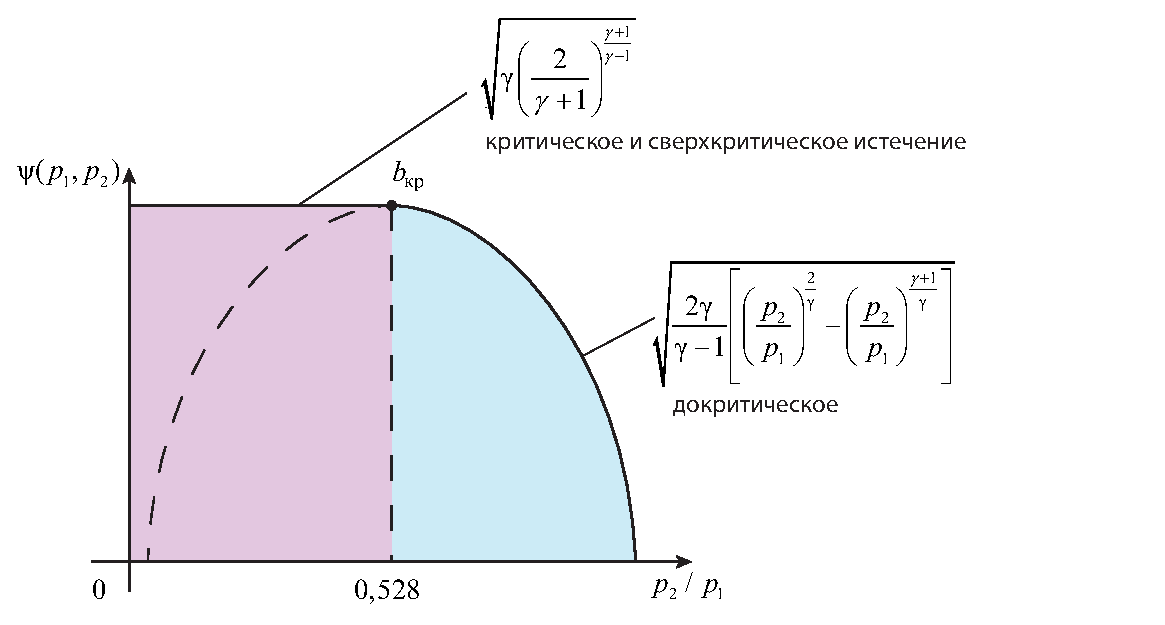
\includegraphics{part2/critical_gas_flow_chart.eps}
    }
    \caption{График расходной функции $\psi(p_1, p_2)$}
    \label{fig:ch2/mass_flow_function}
\end{figure}

На графике отчетливо видны две области: докритическое и закритическое течение, разделенные точкой
критического отношения давлений $b_{кр}$.

В области докритического течения ($p_2/p_1 > b_{кр}$) расход зависит от отношения давлений и
описывается нелинейной функцией. Здесь наблюдается плавное увеличение расхода с уменьшением отношения давлений.

В закритической области ($p_2/p_1 \leq b_{кр}$) расход достигает максимального
значения и остается постоянным независимо от дальнейшего снижения отношения давлений.
Это явление связано с достижением скорости потока воздуха
в самом узком сечении распределителя скорости звука.

Критическая точка $b_{кр}$ соответствует условию, при котором скорость потока
воздуха в самом узком сечении распределителя достигает скорости звука. Для
воздуха при нормальных условиях значение $b_{кр}$ составляет приблизительно \num{0.528}.
Эффективная площадь проходного сечения $F_\text{др}$ зависит от
положения запорно-регулирующего элемента распределителя и может
быть представлена как функция управляющего сигнала $u$:
\begin{equation}
    F_\text{др} = F_{max} \cdot f(u),
\end{equation}
где $F_{max} = F_\text{пр}$ -- максимальная эффективная площадь проходного сечения;
$f(u)$ -- функция, описывающая зависимость площади от управляющего сигнала.

В данной работе используется линейная зависимость площади проходного сечения от управляющего сигнала.
\begin{equation}
    f(u) = F_{max} \cdot u.
\end{equation}

Тогда уравнение массового расхода принимает вид:
\begin{equation}
\label{eq:ch2/mass_flow}
    G = \psi(p_1, p_2) \cdot C_d F_{max} \cdot u \frac{p_1}{\sqrt{RT_\text{вх}}}.
\end{equation}

Представленная модель массового расхода позволяет точно описать процесс истечения
воздуха через дискретный распределитель в различных режимах работы
пневмопривода. Учет нелинейного характера расходной функции и
влияния критического отношения давлений особенно важен при анализе динамики
системы и разработке алгоритмов управления, обеспечивающих высокую точность
и быстродействие электропневматического привода.

\subsection{Динамика переключения распределителей}\label{sec:ch2/sec3/subsec2}

Процесс переключения дискретного распределителя характеризуется
определенной динамикой, которую необходимо учитывать для точного моделирования поведения
системы. Динамика переключения может быть описана дифференциальным уравнением первого порядка:
\begin{equation}
\label{eq:ch2/switching_dynamics}
    \tau \frac{du}{dt} + u = u_{зад},
\end{equation}
где:
$u$ -- текущее положение запорно-регулирующего элемента;
$u_{зад}$ -- заданное положение (0 или 1 для дискретного распределителя);
$\tau$ -- постоянная времени переключения.

Учет динамики переключения позволяет моделировать такие эффекты, как задержка
срабатывания и дребезг контактов, которые могут оказывать
существенное влияние на поведение системы,
особенно при высокочастотном управлении.

Интеграция моделей массового расхода и динамики переключения
в общую математическую модель электропневматического привода
осуществляется путем их включения в уравнения
изменения давлений в полостях пневмоцилиндра \ref{eq:ch2/pressure_system}.

В данной работе использована модель первого порядка для описания динамики переключения
поскольку она обеспечивает достаточно точное описание процесса переключения
и имеет простую структуру.



\section{Адаптация математической модели к эффективному численному расчету на ЭВМ}\label{sec:ch2/sec4}

Эффективное численное моделирование динамики электропневматического привода требует
оптимизации математической модели для выполнения расчетов на ЭВМ.
Данный этап критически важен для обеспечения высокой производительности
вычислений при проведении многочисленных итераций в задачах оптимизации,
анализа чувствительности и робастности системы управления.

Основные цели оптимизации математической модели включают:

\begin{enumerate}
    \item Снижение вычислительной сложности уравнений;
    \item Уменьшение времени выполнения расчетов;
    \item Повышение численной устойчивости алгоритмов;
    \item Эффективное использование параллельных вычислительных архитектур.
\end{enumerate}

Для достижения этих целей будут применены следующие методы:

\begin{enumerate}
    \item Векторизация уравнений;
    \item Упрощение и линеаризация нелинейных выражений;
    \item Предварительное вычисление констант и коэффициентов;
\end{enumerate}
\subsection{Векторизация уравнений}\label{sec:ch2/sec4/subsec1}
Векторизация уравнений представляет собой эффективный метод оптимизации вычислений,
позволяющий использовать преимущества SIMD-инструкций (Single Instruction, Multiple Data)
современных процессоров. Данный подход особенно актуален для математической
модели электропневматического привода с дискретными распределителями, где многие операции могут быть выполнены
параллельно \cite*{eichenberger2004simd} над несколькими элементами данных.

Основная идея векторизации заключается в преобразовании скалярных операций в
векторные, что позволяет обрабатывать несколько элементов данных
одновременно \cite*{nuzman2011vaporsimd}. В контексте рассматриваемой модели это означает переход от
поэлементных вычислений к операциям над векторами и матрицами.
Процесс векторизации начинается с представления состояния системы
в виде единого вектора. Для электропневматического привода
вектор состояния может быть записан как:

\begin{equation}
\label{eq:ch2/state_vector}
    \mathbf{y} = [x, v, p_1, p_2, T_1, T_2, u_1, u_2, u_3, u_4]^T.
\end{equation}

Векторизованная форма уравнения движения поршня \eqref{eq:ch2/eq8} может быть представлена следующим образом:

\begin{equation}
\label{eq:ch2/vec_motion}
    M\ddot{x} = \mathbf{F}^T\mathbf{p} - p_\text{атм}(\mathbf{F}^T\mathbf{1}) - R_\text{тр}(\dot{x}) - R_\text{оп}(x, \dot{x}),
\end{equation}
где $\mathbf{F} = [F_1, -F_2]^T$ -- вектор эффективных площадей поршня;
$\mathbf{p} = [p_1, p_2]^T$ -- вектор давлений в полостях цилиндра;
$\mathbf{1} = [1, 1]^T$ - единичный вектор.

Уравнения изменения давлений в полостях \eqref{eq:ch2/final_pressure_system} могут быть векторизованы следующим образом:
\begin{equation}
\label{eq:ch2/vec_pressure}
    \dot{\mathbf{p}} = \frac{\gamma}{\mathbf{V}(\mathbf{x})} \odot (R\mathbf{T} \odot \mathbf{G} - \mathbf{p} \odot (\mathbf{F}\dot{x})),
\end{equation}
где $\odot$ обозначает поэлементное умножение векторов;
$\mathbf{T} = [T_1, T_2]^T$ -- вектор температур в полостях;
$\mathbf{G} = [G_1, G_2]^T$ -- вектор суммарных массовых расходов для каждой полости;
$\mathbf{V}(\mathbf{x}) = [V_1(x), V_2(x)]^T$ -- вектор-функция объемов полостей.

Уравнения изменения температур \eqref{eq:ch2/energy_balance_final} также могут быть представлены в векторной форме:
\begin{equation}
\label{eq:ch2/vec_temperature}
    \dot{\mathbf{T}} = \frac{\gamma-1}{\mathbf{m}C_v} \odot (R\mathbf{T} \odot \mathbf{G} \pm \mathbf{p} \odot (\mathbf{F}\dot{x})),
\end{equation}
где $\mathbf{m} = [m_1, m_2]^T$ -- вектор масс воздуха в полостях.

Динамика переключения распределителей \eqref{eq:ch2/switching_dynamics} может быть векторизована для всех четырех распределителей одновременно:
\begin{equation}
\label{eq:ch2/vec_switching}
    \tau \dot{\mathbf{u}} + \mathbf{u} = \mathbf{u}_\text{зад},
\end{equation}
где $\mathbf{u} = [u_1, u_2, u_3, u_4]^T$ -- вектор текущих положений запорно-регулирующих элементов распределителей;
$\mathbf{u}_\text{зад}$ -- вектор заданных положений.

Для расчета массовых расходов через распределители можно использовать векторизованную форму уравнения массового расхода:
\begin{equation}
\label{eq:ch2/vec_mass_flow}
    \mathbf{G} = \psi(\mathbf{p}_\text{вх}, \mathbf{p}_\text{вых}) \odot \mathbf{C}_d \odot \mathbf{F}_\text{пр} \odot \mathbf{u} \odot \frac{\mathbf{p}_\text{вх}}{\sqrt{R\mathbf{T}_\text{вх}}},
\end{equation}
где $\psi(\mathbf{p}_\text{вх}, \mathbf{p}_\text{вых})$ -- векторизованная расходная функция;
$\mathbf{C}_d$ и $\mathbf{F}_\text{пр}$ -- векторы коэффициентов расхода и эффективных площадей проходных сечений распределителей соответственно.

Применение векторизации позволяет эффективно использовать SIMD-инструкции процессора,
что приводит к значительному ускорению вычислений. В зависимости от архитектуры процессора и
специфики реализации, ускорение может достигать 2-4 раза \cite*{tian2013simd} по сравнению с исходной скалярной версией.

\subsection{Оптимизация нелинейных функций}\label{sec:ch2/sec4/subsec2}

Так же важным этапом оптимизации является упрощение и линеаризация нелинейных функций,
которые могут оказывать существенное влияние на вычислительную сложность модели и деаль ее
жесткой. В контексте электропневматического привода, к нелинейным функцям относятся экспоненциальная
функция в модели трения, функция sign, реакция упоров и условные операции.

Для оптимизации вычисления экспоненциальной функции в модели трения предлагается использовать аппроксимацию Паде.
Данный метод обеспечивает высокую точность аппроксимации при сравнительно низкой вычислительной
сложности. Аппроксимация Паде для экспоненциальной функции может быть представлена в виде:

\begin{equation}
    e^x \approx \frac{1 + \frac{x}{2} + \frac{x^2}{10} + \frac{x^3}{120}}{1 - \frac{x}{2} + \frac{x^2}{10} - \frac{x^3}{120}}.
\end{equation}

Данная аппроксимация обеспечивает высокую точность в диапазоне $x \in [-2,5; 2,5]$,
что достаточно для моделирования эффекта Штрибека в рассматриваемой системе.

Реакция упоров, обычно моделируемая с использованием условных операций, может быть
оптимизирована применением непрерывной аппроксимации:

\begin{equation}
    R_\text{оп} = k_\text{оп}(x - x_\text{мин})\cdot S(x - x_\text{мин}) + k_\text{оп}(x - x_\text{макс})\cdot S(x - x_\text{макс}),
\end{equation}
где $S(x)$ -- сглаживающая функция, например:

\begin{equation}
    S(x) = \frac{1}{1 + e^{-\alpha x}},
\end{equation}
где $\alpha$ -- параметр, определяющий крутизну перехода.

Для оптимизации условных операций в модели предлагается
использовать непрерывные аппроксимации. Например, функция
максимума может быть аппроксимирована как:

\begin{equation}
    \max(a, b) \approx \frac{a + b + \sqrt{(a - b)^2 + \varepsilon}}{2},
\end{equation}
где $\varepsilon$ -- малое положительное число, обеспечивающее гладкость функции.

Применяя предложенные оптимизации, уравнения реакции упоров и силы трения могут быть представлены в виде:

\begin{equation}
    \begin{alignedat}{2}
        g(v) & = \left[R_\text{к} + (R_\text{с} - R_\text{к})\frac{1 + \frac{z}{2} + \frac{z^2}{10} + \frac{z^3}{120}}{1 - \frac{z}{2} + \frac{z^2}{10} - \frac{z^3}{120}}\right] \\
        R_\text{оп} & = k_\text{оп}(x - x_\text{мин})\cdot \frac{1}{1 + e^{-\alpha(x - x_\text{мин})}} + k_\text{оп}(x - x_\text{макс})\cdot \frac{1}{1 + e^{-\alpha(x - x_\text{макс})}},
    \end{alignedat}
\end{equation}

\subsection{Аналитическое вычисление якобиана для численного решения ОДУ}\label{sec:ch2/sec5/subsec3}

В контексте оптимизации математической модели пневматического привода была реализована процедура аналитического
вычисления матрицы Якоби для повышения эффективности численного интегрирования. Данный подход позволяет
существенно снизить вычислительные затраты и повысить численную стабильность решения системы дифференциальных уравнений.

Якобиан системы определяется как матрица частных производных:

\begin{equation}
\label{eq:ch2/jacobian_matrix}
    J = \frac{\partial \mathbf{f}}{\partial \mathbf{y}} =
    \begin{pmatrix}
        \frac{\partial f_1}{\partial y_1}    & \frac{\partial f_1}{\partial y_2}    & \cdots & \frac{\partial f_1}{\partial y_{10}}    \\
        \frac{\partial f_2}{\partial y_1}    & \frac{\partial f_2}{\partial y_2}    & \cdots & \frac{\partial f_2}{\partial y_{10}}    \\
        \vdots                               & \vdots                               & \ddots & \vdots                                  \\
        \frac{\partial f_{10}}{\partial y_1} & \frac{\partial f_{10}}{\partial y_2} & \cdots & \frac{\partial f_{10}}{\partial y_{10}}
    \end{pmatrix}
\end{equation}

где $\mathbf{f}$ -- вектор-функция правых частей системы дифференциальных уравнений.


Рассмотрим вычисление элементов матрицы Якоби для каждого уравнения системы:

\paragraph{Уравнение движения поршня}
Для уравнения движения поршня $\dot{x} = v$ имеем:
\begin{equation}
\label{eq:ch2/jacobian_motion}
    \begin{aligned}
        \frac{\partial \dot{x}}{\partial x}   & = 0                          \\
        \frac{\partial \dot{x}}{\partial v}   & = 1                          \\
        \frac{\partial \dot{x}}{\partial y_i} & = 0, \quad i = 3, \ldots, 10
    \end{aligned}
\end{equation}

\paragraph{Уравнение ускорения поршня}
Для уравнения ускорения поршня:
\begin{equation}
\label{eq:ch2/jacobian_acceleration}
    \begin{aligned}
        \frac{\partial \dot{v}}{\partial x}   & = -\frac{1}{M}\left(\frac{\partial R_\text{тр}}{\partial x} + \frac{\partial R_\text{оп}}{\partial x}\right) \\
        \frac{\partial \dot{v}}{\partial v}   & = -\frac{1}{M}\left(\frac{\partial R_\text{тр}}{\partial v} + \frac{\partial R_\text{оп}}{\partial v}\right) \\
        \frac{\partial \dot{v}}{\partial p_1} & = \frac{F_1}{M}                                                                                              \\
        \frac{\partial \dot{v}}{\partial p_2} & = -\frac{F_2}{M}                                                                                             \\
        \frac{\partial \dot{v}}{\partial y_i} & = 0, \quad i = 5, \ldots, 10
    \end{aligned}
\end{equation}
где частные производные силы трения и реакции опоры вычисляются на основе их моделей
\eqref{eq:ch2/friction_force} и \eqref{eq:ch2/support_reaction} соответственно.

\paragraph{Уравнения изменения давлений}
Для уравнений изменения давлений в полостях цилиндра:
\begin{equation}
\label{eq:ch2/jacobian_pressure}
    \begin{aligned}
        \frac{\partial \dot{p_i}}{\partial x}   & = -\frac{\gamma p_i}{V_i^2}\frac{\partial V_i}{\partial x}(RT_iG_i - p_iF_iv) + \frac{\gamma}{V_i}\left(RT_i\frac{\partial G_i}{\partial x} - F_iv\frac{\partial p_i}{\partial x} - p_iF_i\frac{\partial v}{\partial x}\right) \\
        \frac{\partial \dot{p_i}}{\partial v}   & = \frac{\gamma}{V_i}\left(RT_i\frac{\partial G_i}{\partial v} - p_iF_i\right)                                                                                                                                                  \\
        \frac{\partial \dot{p_i}}{\partial p_i} & = \frac{\gamma}{V_i}\left(RT_i\frac{\partial G_i}{\partial p_i} - F_iv\right)                                                                                                                                                  \\
        \frac{\partial \dot{p_i}}{\partial T_i} & = \frac{\gamma}{V_i}\left(RG_i + RT_i\frac{\partial G_i}{\partial T_i}\right)                                                                                                                                                  \\
        \frac{\partial \dot{p_i}}{\partial u_j} & = \frac{\gamma RT_i}{V_i}\frac{\partial G_i}{\partial u_j}, \quad j = 1, \ldots, 4
    \end{aligned}
\end{equation}
где $i = 1, 2$ для левой и правой полостей соответственно.

\paragraph{Уравнения изменения температур}
Аналогично для уравнений изменения температур:
\begin{equation}
\label{eq:ch2/jacobian_temperature}
    \begin{aligned}
        \frac{\partial \dot{T_i}}{\partial x}   & = \frac{\gamma-1}{m_iC_v}\left(R\frac{\partial (T_iG_i)}{\partial x} \pm \frac{\partial (p_iF_iv)}{\partial x}\right) \\
        \frac{\partial \dot{T_i}}{\partial v}   & = \frac{\gamma-1}{m_iC_v}\left(R\frac{\partial (T_iG_i)}{\partial v} \pm p_iF_i\right)                                \\
        \frac{\partial \dot{T_i}}{\partial p_i} & = \frac{\gamma-1}{m_iC_v}\left(R\frac{\partial (T_iG_i)}{\partial p_i} \pm F_iv\right)                                \\
        \frac{\partial \dot{T_i}}{\partial T_i} & = \frac{\gamma-1}{m_iC_v}\left(RG_i + RT_i\frac{\partial G_i}{\partial T_i}\right)                                    \\
        \frac{\partial \dot{T_i}}{\partial u_j} & = \frac{(\gamma-1)RT_i}{m_iC_v}\frac{\partial G_i}{\partial u_j}, \quad j = 1, \ldots, 4
    \end{aligned}
\end{equation}

\paragraph{Уравнения динамики переключения распределителей}
Для уравнений динамики переключения распределителей:
\begin{equation}
\label{eq:ch2/jacobian_valves}
    \begin{aligned}
        \frac{\partial \dot{u_i}}{\partial u_i} & = -\frac{1}{\tau}     \\
        \frac{\partial \dot{u_i}}{\partial y_j} & = 0, \quad j \neq i+6
    \end{aligned}
\end{equation}
где $i = 1, \ldots, 4$ для каждого распределителя.

Для вычисления частных производных массового расхода $\partial G_i/\partial y_j$ необходимо учитывать нелинейную
зависимость расходной функции $\psi(p_1, p_2)$ от давлений.

Рассмотрим производные расходной функции по давлениям:
\begin{equation}
\label{eq:ch2/flow_function_derivatives}
    \begin{alignedat}{6}
        \frac{\partial \psi}{\partial p_1} & = \begin{cases}
                                                   -\frac{1}{p_1}\frac{\gamma+1}{\gamma-1}\left(\frac{p_2}{p_1}\right)^{\frac{2}{\gamma}}\left[1 - \left(\frac{p_2}{p_1}\right)^{\frac{\gamma-1}{\gamma}}\right]\frac{1}{\psi}, & \text{если } \frac{p_2}{p_1} > b_\text{кр}    \\
                                                   0,                                                                                                                                                                           & \text{если } \frac{p_2}{p_1} \leq b_\text{кр} \\
                                               \end{cases} \\
        \frac{\partial \psi}{\partial p_2} & = \begin{cases}
                                                   \frac{1}{p_2}\frac{\gamma+1}{\gamma-1}\left(\frac{p_2}{p_1}\right)^{\frac{2}{\gamma}-1}\left[1 - \left(\frac{p_2}{p_1}\right)\right]\frac{1}{\psi}, & \text{если } \frac{p_2}{p_1} > b_\text{кр}    \\
                                                   0,                                                                                                                                                  & \text{если } \frac{p_2}{p_1} \leq b_\text{кр}
                                               \end{cases}
    \end{alignedat}
\end{equation}

Теперь, используя эти производные, можно вычислить частные производные массового расхода по переменным состояния системы. Для примера рассмотрим производную массового расхода по давлению в первой полости цилиндра:
\begin{equation}
\label{eq:ch2/mass_flow_derivative}
    \frac{\partial G_1}{\partial p_1} = C_d F_\text{пр} u_1 \left(\frac{\partial \psi}{\partial p_1} \cdot \frac{p_1}{\sqrt{RT_1}} + \psi \cdot \frac{1}{\sqrt{RT_1}}\right)
\end{equation}

Аналогичным образом вычисляются производные по другим переменным состояния. Для производных по температуре и положениям запорно-регулирующих элементов распределителей имеем:
\begin{equation}
\label{eq:ch2/mass_flow_derivative_T}
    \begin{aligned}
        \frac{\partial G_1}{\partial T_1} & = -\frac{1}{2} C_d F_\text{пр} u_1 \psi \frac{p_1}{\sqrt{RT_1^3}} \\
        \frac{\partial G_1}{\partial u_1} & = C_d F_\text{пр} \psi \frac{p_1}{\sqrt{RT_1}}
    \end{aligned}
\end{equation}

Полная матрица Якоби формируется путем объединения всех вычисленных частных производных в
соответствии с их позициями в векторе состояния системы \eqref{eq:ch2/state_vector}.

Применение якобиана для в методах численных численного интегрирования, таких как
BDF (Backward Differentiation Formula) и Radau, позволяет уменьшить количество вычислений
и повысить численную стабильность. В частности, использование якобиана позволяет
уменьшить количество вычислений правых частей системы, что особенно важно для жестких систем.

\section{Реализация математической модели}\label{sec:ch2/sec5}

Сведем полученные выражения в единую систему:

\begin{equation}\label{eq:ch2/final_system}
    \begin{cases}
        \begin{alignedat}{2}
            \dot{x}               & = v                                                                                                                                                                                                   \\
            M\dot{v}              & = \mathbf{F}^T\mathbf{p} - p_\text{атм}(\mathbf{F}^T\mathbf{1}) - R_\text{тр}(v) - R_\text{оп}(x, v)                                                                                                  \\
            \dot{\mathbf{p}}      & = \frac{\gamma}{\mathbf{V}(\mathbf{x})} \odot (R\mathbf{T} \odot \mathbf{G} - \mathbf{p} \odot (\mathbf{F}v))                                                                                         \\
            \dot{\mathbf{T}}      & = \frac{\gamma-1}{\mathbf{m}C_v} \odot (R\mathbf{T} \odot \mathbf{G} \pm \mathbf{p} \odot (\mathbf{F}v))                                                                                              \\
            \mathbf{u}_\text{зад} & = \tau \dot{\mathbf{u}} + \mathbf{u}                                                                                                                                                                  \\
            \mathbf{G}            & = \psi(\mathbf{p}_\text{вх}, \mathbf{p}_\text{вых}) \odot \mathbf{C}_d \odot \mathbf{F}_\text{пр} \odot \mathbf{u} \odot \frac{\mathbf{p}_\text{вх}}{\sqrt{R\mathbf{T}_\text{вх}}}                    \\
            R_\text{тр} &= \sigma_0 z + \sigma_1 \dot{z} + \sigma_2 v                                                                                                                              \\
            \dot{z} &= v - \frac{\sigma_0 |v|}{g(v)}z \\
            R_\text{оп}           & = k_\text{оп}(x - x_\text{мин})\cdot \frac{1}{1 + e^{-\alpha(x - x_\text{мин})}} + k_\text{оп}(x - x_\text{макс})\cdot \frac{1}{1 + e^{-\alpha(x - x_\text{макс})}}                                   \\
        \end{alignedat}
    \end{cases}
\end{equation}

Представим данную систему в виде функциональной блок-схемы, представленной на рисунке \ref{fig:ch2/block_diagram}.

\begin{figure}[ht]
    \centerfloat{
        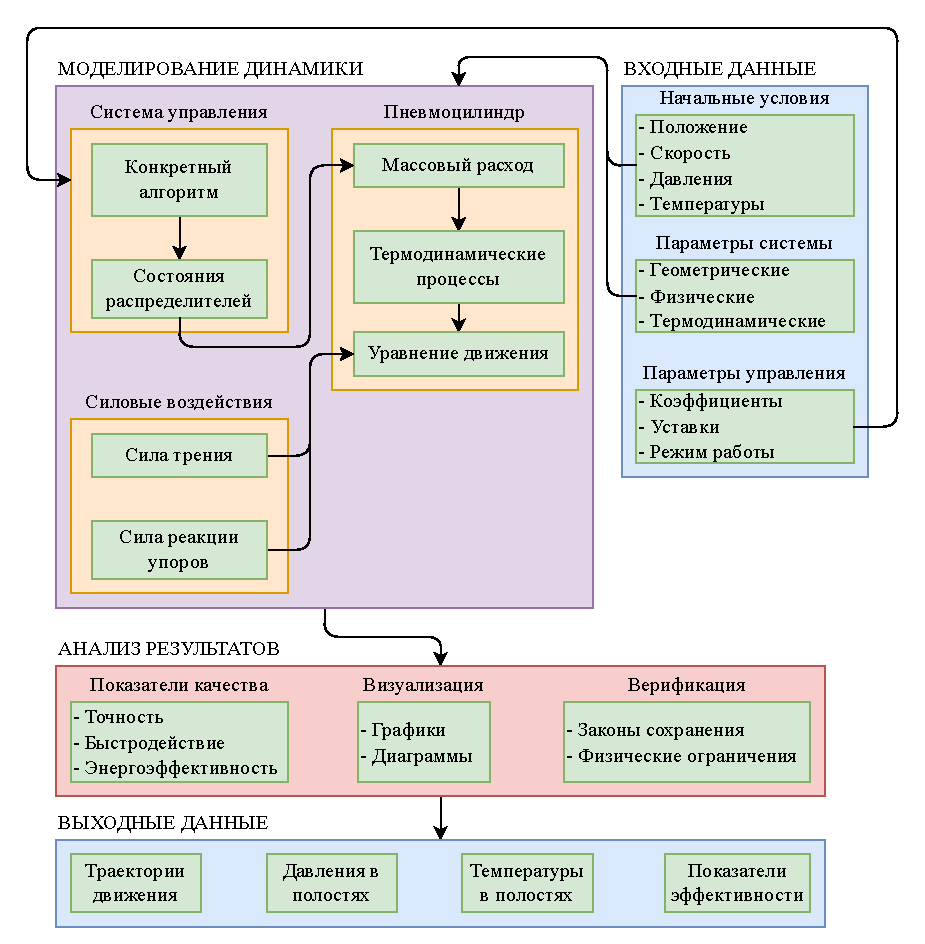
\includegraphics[]{part2/diagrams/pneumatic_actuator_functional_block_diagram.pdf}
    }
    \caption{Функциональная блок-схема математической модели электропневматического привода}
    \label{fig:ch2/block_diagram}
\end{figure}

В процессе исследования осуществлена программная реализация математической модели пневматического привода с применением объектно-ориентированного подхода.
При разработке программного комплекса использован язык программирования Python, обеспечивающий необходимую функциональность для численного моделирования и
обработки результатов. Архитектура программного комплекса базируется на принципах модульности и инкапсуляции, что обеспечивает высокую степень гибкости при
модификации отдельных компонентов системы.

Центральным элементом реализации является класс \texttt{PneumaticCylinder}, инкапсулирующий математическую модель пневматического привода.
В данном классе реализована система дифференциальных уравнений, описывающих динамику привода, включая уравнения движения поршня,
термодинамические процессы в рабочих полостях и динамику переключения распределителей. Математическая модель дополнена отдельными
классами для описания нелинейных эффектов: \texttt{FrictionModel} -- для моделирования сил трения и \texttt{StopForce} -- для учета ограничений хода поршня.

Численное интегрирование системы дифференциальных уравнений осуществляется с использованием метода BDF (Backward Differentiation Formula),
реализованного в библиотеке \texttt{scipy.integrate}. Выбор данного метода обусловлен жёсткостью исследуемой системы дифференциальных
уравнений. Для повышения эффективности численного интегрирования реализовано аналитическое вычисление матрицы Якоби, что позволяет существенно
сократить вычислительные затраты и повысить численную стабильность решения.

Визуализация результатов моделирования реализована с применением библиотеки Matplotlib, обеспечивающей
построение графиков временных зависимостей основных параметров системы: перемещения и скорости поршня, давлений и температур
в полостях цилиндра, состояний распределителей. При этом программный комплекс предусматривает возможность экспорта результатов
в различные форматы для последующей обработки и анализа.

Разработанная программная реализация обеспечивает возможность эффективного проведения вычислительных экспериментов,
параметрической оптимизации и анализа динамических характеристик пневматического привода. Модульная структура программного
комплекса позволяет легко модифицировать отдельные компоненты системы и интегрировать новые алгоритмы управления.

\section{Верификация математической модели}\label{sec:ch2/sec6}
Верификация математической модели  представляет собой неотъемлемый этап разработки, направленный на подтверждение адекватности
и точности полученного математического описания. Процесс верификации включает в себя комплекс методов и подходов,
позволяющих оценить соответствие модели реальному объекту в рамках принятых допущений и ограничений.

Основной целью верификации является подтверждение способности модели корректно отражать физические процессы,
происходящие в электропневматическом приводе, и обеспечивать достоверные результаты при решении задач анализа и синтеза систем управления.
В отсутствие экспериментальных данных, предварительная верификация базируется на теоретическом анализе,
численном моделировании.

Верификация данных происходила на основе следующих параметров модели, которые согласованны
с характерными параметрами экпериментального стенда и пердставлены в
таблице \ref{tab:ch2/extended_parameters}.

\begin{table}[h]
    \centering
    \caption{Расширенные параметры моделирования электропневматического привода}
    \small
    \begin{tabular}{lccl}
        \textbf{Параметр}                & \textbf{Обозначение}                      & \textbf{Значение}     & \textbf{Размерность} \\
        \midrule
        Масса подвижных частей           & $M$                                       & 6.0                   & кг                   \\
        Ход поршня                       & $L$                                       & 0.3                   & м                    \\
        Диаметр поршня                   & $D_\text{п}$                              & 0.032                 & м                    \\
        Диаметр штока                    & $d_\text{шт}$                             & 0.012                 & м                    \\
        Площадь поршня со стороны штока  & $F_2 = \pi(D_\text{п}^2-d_\text{шт}^2)/4$ & $7.07 \times 10^{-4}$ & м$^2$                \\
        Площадь поршня со стороны крышки & $F_1 = \pi D_\text{п}^2/4$                & $8.04 \times 10^{-4}$ & м$^2$                \\
        Давление питания                 & $p_\text{п}$                              & $6 \times 10^5$       & Па                   \\
        Атмосферное давление             & $p_\text{атм}$                            & $1 \times 10^5$       & Па                   \\
        Газовая постоянная воздуха       & $R$                                       & 287                   & Дж/(кг$\cdot$К)      \\
        Температура воздуха              & $T_\text{атм}$                            & 293                   & К                    \\
        Показатель адиабаты              & $\gamma$                                  & 1.4                   & -                    \\
        Коэффициент расхода              & $C_d$                                     & 0.7                   & -                    \\
        Эффективная площадь клапана      & $A_v$                                     & $1.2 \times 10^{-6}$  & м$^2$                \\
        \midrule
        \multicolumn{4}{l}{\textbf{Параметры силы трения:}}                                                                         \\
        \midrule
        Сила сухого трения               & $F_c$                                     & 50                    & Н                    \\
        Сила трения покоя                & $F_s$                                     & 60                    & Н                    \\
        Коэффициент вязкого трения       & $\sigma_2$                                & 100                   & Н$\cdot$с/м          \\
        Скорость Штрибека                & $v_s$                                     & 0.01                  & м/с                  \\
        Показатель степени Штрибека      & $\delta$                                  & 2                     & -                    \\
        \midrule
        \multicolumn{4}{l}{\textbf{Параметры реакции опор:}}                                                                        \\
        \midrule
        Коэффициент жесткости опоры      & $k_\text{оп}$                             & $1 \times 10^6$       & Н/м                  \\
        Коэффициент демпфирования опоры  & $b_\text{оп}$                             & 1000                  & Н$\cdot$с/м          \\
        Координата нижнего упора         & $x_\text{мин}$                            & 0                     & м                    \\
        Координата верхнего упора        & $x_\text{макс}$                           & 0.3                   & м                    \\
        \midrule
    \end{tabular}
    \label{tab:ch2/extended_parameters}
\end{table}

\subsection{Теоретические основы верификации}\label{sec:ch2/sec6/subsec1}
Процесс верификации основывается на следующих ключевых принципах:

\begin{enumerate}
    \item Принцип физической непротиворечивости, требующий соответствия модели фундаментальным законам механики и пневматики;
    \item Принцип математической корректности, предполагающий отсутствие ошибок в формулировке уравнений и их решении;
    \item Принцип консервативности, обеспечивающий выполнение законов сохранения массы и энергии в модели;
    \item Принцип устойчивости решения, гарантирующий сходимость численных методов при различных начальных условиях и параметрах системы.
\end{enumerate}

Методологический базис верификации включает:

\begin{enumerate}
    \item Аналитический анализ структуры модели и ее соответствия физическим законам;
    \item Численное моделирование с исследованием сходимости и устойчивости решения;
    \item Анализ предельных случаев и упрощенных режимов работы системы;
    \item Оценку чувствительности модели к вариациям параметров.
\end{enumerate}

Математически процесс верификации может быть формализован как задача минимизации функционала
ошибки между результатами моделирования и теоретическими предсказаниями для известных частных случаев:
\begin{equation}
    J = \min_{\theta} \sum_{i=1}^{N} \left| f_{\text{модель}}(x_i, \theta) - f_{\text{теория}}(x_i) \right|^2,
\end{equation}
где $f_{\text{модель}}$ -- функция, описывающая выход модели;
$f_{\text{теория}}$ -- теоретически предсказанное значение;
$x_i$ -- входные параметры;
$\theta$ -- параметры модели;
$N$ -- количество точек сравнения.

Выбор методов верификации обусловлен спецификой исследуемой системы и включает:

\begin{enumerate}
    \item Проверку размерностей и единиц измерения всех величин в уравнениях модели.
    \item    Анализ асимптотического поведения модели при предельных значениях параметров.
    \item Исследование сходимости численного решения при измельчении шага интегрирования.
    \item Оценку энергетического баланса системы и соблюдения закона сохранения массы.
\end{enumerate}

\subsection{Проверка маетматической корректности}\label{sec:ch2/sec6/subsec2}

Проверка математической корректности модели электропневматического привода с дискретными распределителями осуществляется посредством следующих процедур:

\begin{enumerate}
    \item Анализ размерностей и единиц измерения;
    \item Верификация согласованности уравнений с законами сохранения;
    \item Оценка физической непротиворечивости уравнений;
    \item Анализ непрерывности и дифференцируемости функций.
\end{enumerate}

Каждая процедура направлена на выявление потенциальных ошибок в математическом описании
системы и обеспечение соответствия модели фундаментальным физическим принципам.

Основные этапы проверки математической корректности модели подробнее:

\paragraph{Анализ размерностей и единиц измерения.}

Проверка согласованности размерностей всех величин, входящих в уравнения модели, осуществляется с использованием метода анализа размерностей. Для каждого уравнения модели выполняется проверка:
\begin{equation}
    [LHS] = [RHS],
\end{equation}
где $[LHS]$ и $[RHS]$ -- размерности левой и правой частей уравнения соответственно.

\paragraph{Верификация согласованности уравнений с законами сохранения.}

Проверяется выполнение законов сохранения массы и энергии. Для закона сохранения массы в пневматической системе:

\begin{equation}
    \frac{d}{dt}(m_1 + m_2) = \dot{m}_\text{вх} - \dot{m}_\text{вых},
\end{equation}

где $m_1$ и $m_2$ -- массы воздуха в первой и второй полостях пневмоцилиндра соответственно;
$\dot{m}_\text{вх}$ -- суммарный массовый расход воздуха, поступающего в систему
$\dot{m}_\text{вых}$ -- суммарный массовый расход воздуха, выходящего из системы.

Для проверки этого закона необходимо вычислить изменение общей массы воздуха в системе и сравнить
его с интегралом разности входящих и выходящих массовых расходов:

\begin{equation}
    \Delta m_\text{общ} = \int_{t_0}^{t_1} (\dot{m}_\text{вх} - \dot{m}_\text{вых}) dt,
\end{equation}

Для закона сохранения энергии:
\begin{equation}
    \frac{d}{dt}(E_k + E_p + U) = W_{\text{внеш}} - Q
\end{equation}
где $E_k$ -- кинетическая энергия;
$E_p$ -- потенциальная энергия;
$U$ -- внутренняя энергия;
$W_{\text{внеш}}$ -- работа внешних сил;
$Q$ -- теплота, переданная системе.

\paragraph{Оценка физической непротиворечивости уравнений.}

В рамках оценки физической непротиворечивости уравнений проводится проверка
выполнения второго закона термодинамики для адиабатного процесса, в частности, принципа неубывания энтропии.

Для адиабатной системы изменение энтропии должно удовлетворять неравенству:
\begin{equation}
    \Delta S \geq 0
\end{equation}
где $\Delta S$ -- изменение энтропии системы.

Проверка неубывания энтропии осуществляется следующим образом:

\begin{enumerate}
    \item Вычисление изменения энтропии для каждой полости цилиндра на каждом шаге интегрирования:
          \begin{equation}
              \Delta S_i = m_i c_v \ln\left(\frac{T_{i,k+1}}{T_{i,k}}\right) + m_i R \ln\left(\frac{V_{i,k+1}}{V_{i,k}}\right),
          \end{equation}
          где $m_i$ -- масса газа в i-й полости;
          $c_v$ -- удельная теплоемкость при постоянном объеме;
          $T_{i,k}$ и $V_{i,k}$ -- температура и объем i-й полости на k-м шаге интегрирования.

    \item Расчет производства энтропии за счет необратимых процессов, включая трение и дросселирование газа:
          \begin{equation}
              \Delta S_{\text{irr}} = \frac{F_{\text{тр}} \Delta x}{T_{\text{ср}}} + \sum_j G_j R \ln\left(\frac{p_{\text{вых},j}}{p_{\text{вх},j}}\right),
          \end{equation}
          где $F_{\text{тр}}$ -- сила трения;
          $\Delta x$ -- перемещение;
          $T_{\text{ср}}$ -- средняя температура;
          $G_j$ -- массовый расход через j-й распределитель;
          $p_{\text{вх},j}$ и $p_{\text{вых},j}$ -- давления на входе и выходе j-го распределителя.

    \item Проверка условия неубывания суммарной энтропии системы:
          \begin{equation}
              \Delta S_{\text{total}} = \sum_i \Delta S_i + \Delta S_{\text{irr}} \geq 0.
          \end{equation}
\end{enumerate}

Дополнительно проверяется выполнение уравнения адиабатного процесса для каждой полости:
\begin{equation}
    pV^{\gamma} = \text{const}.
\end{equation}

\subsection{Оценка физичности результатов моделирования}\label{sec:ch2/sec6/subsec4}

\paragraph{Проверка размерностей и единиц измерения.}
Рассматриваются размерности основных физических величин, используемых в модели:

\begin{itemize}
    \item Длина: $ [L] = \text{м}$;
    \item Время: $ [T] = \text{с}$;
    \item Масса: $ [M] = \text{кг}$;
    \item Сила: $ [F] = \text{кг}\cdot\text{м}/\text{с}^2$;
    \item Давление: $ [P] = \text{кг}/(\text{м}\cdot\text{с}^2)$;
    \item Температура: $ [\Theta] = \text{К}$.
\end{itemize}

Анализ размерностей для каждого уравнения системы:
\begin{itemize}
    \item Уравнение движения поршня: $ [M\cdot L/T^2] = [P\cdot L^2] + [F]$;
    \item Уравнение изменения давления: $ [P/T] = [M/(L^2\cdot T^2)] $;
    \item Уравнение изменения температуры: $ [\Theta/T] = [\Theta/T]$;
    \item Уравнение массового расхода: $  [M/T] = [L^2] \cdot [P] / [L/T] = [M/T] $;
    \item Уравнение силы трения: $  [F] = [F] + [F\cdot T/L] \cdot [L/T] = [F] $;
    \item Уравнение реакции опоры: $  [F] = [F/L] \cdot [L] = [F] $;
    \item Уравнение динамики золотников: $  [1] = [1]$.
\end{itemize}


Проведенный анализ подтверждает согласованность размерностей во всех уравнениях математической модели.
Это свидетельствует о корректности формулировки модели с точки зрения физических единиц измерения.

\paragraph{Верификация согласованности уравнений с законами сохранения.}
Исследование энергетического баланса системы и закона сохранения массы проводились
для различных состояний распределителей. В таблице \ref{tab:ch2/valve_states} представлены состояния распределителей,
для которых проводилась верификация.

\begin{table}[h]
    \centering
    \caption{Состояния распределителей для верификации модели и начальных условий давлений}
    \begin{tabular}{l|c|c|c|c|c|c}
        \midrule
        № описания & $u_1$ & $u_2$ & $u_3$ & $u_4$ & $p_1\text{, Па}$ & $p_2\text{, Па}$ \\
        \midrule
        1          & 1     & 0     & 0     & 1     & \num{1e5}        & \num{1e5}        \\
        \hline
        2          & 1     & 0     & 0     & 0     & \num{1e5}        & \num{1e5}        \\
        \hline
        3          & 0     & 0     & 0     & 1     & \num{5e5}        & \num{1e5}        \\
        \hline
        4          & 0     & 1     & 1     & 0     & \num{1e5}        & \num{1e5}        \\
        \hline
        5          & 0     & 0     & 1     & 0     & \num{1e5}        & \num{1e5}        \\
        \hline
        6          & 0     & 1     & 0     & 0     & \num{1e5}        & \num{5e5}        \\
        \midrule
    \end{tabular}
    \label{tab:ch2/valve_states}
\end{table}

Исследования проводились для шести режимов работы,
каждый из которых характеризуется уникальной конфигурацией клапанов и соответствующим воздействием на движение поршня.
Режим 1 обеспечивает максимальное ускорение в положительном направлении посредством одновременной подачи сжатого воздуха
в переднюю полость пневмоцилиндра и сброса воздуха из задней полости в атмосферу, создавая максимальный перепад давлений.
В режиме 2 реализуется умеренное ускорение в положительном направлении за счет подачи сжатого воздуха только в переднюю полость
при изолированной задней полости, что приводит к более плавному увеличению давления. Режим 3 предназначен для замедления при
движении в положительном направлении: передняя полость изолируется, а из задней осуществляется выпуск воздуха в атмосферу,
снижая противодействующее давление. Режим 4, являясь обратным по отношению к первому, обеспечивает максимальное ускорение
в отрицательном направлении путем подачи сжатого воздуха в заднюю полость и выпуска воздуха из передней. Режим 5 аналогичен
второму, но для противоположного направления движения: сжатый воздух подается только в заднюю полость при изолированной передней.
Режим 6 симметричен третьему и предназначен для замедления при движении в отрицательном направлении: задняя полость изолируется,
а из передней осуществляется выпуск воздуха.

Графики на рисунке \ref{fig:ch2/energy_balance} демонстрируют энергетический баланс системы для режима 2. Остальные
режимы представлены в приложении к \fixme{диссертации}. Как видно из графиков, энергетический баланс системы соблюдается
для всех рассмотренных режимов, что свидетельствует о соблюдении закона сохранения энергии и массы в модели.

\begin{figure}[ht]
    \centerfloat {
        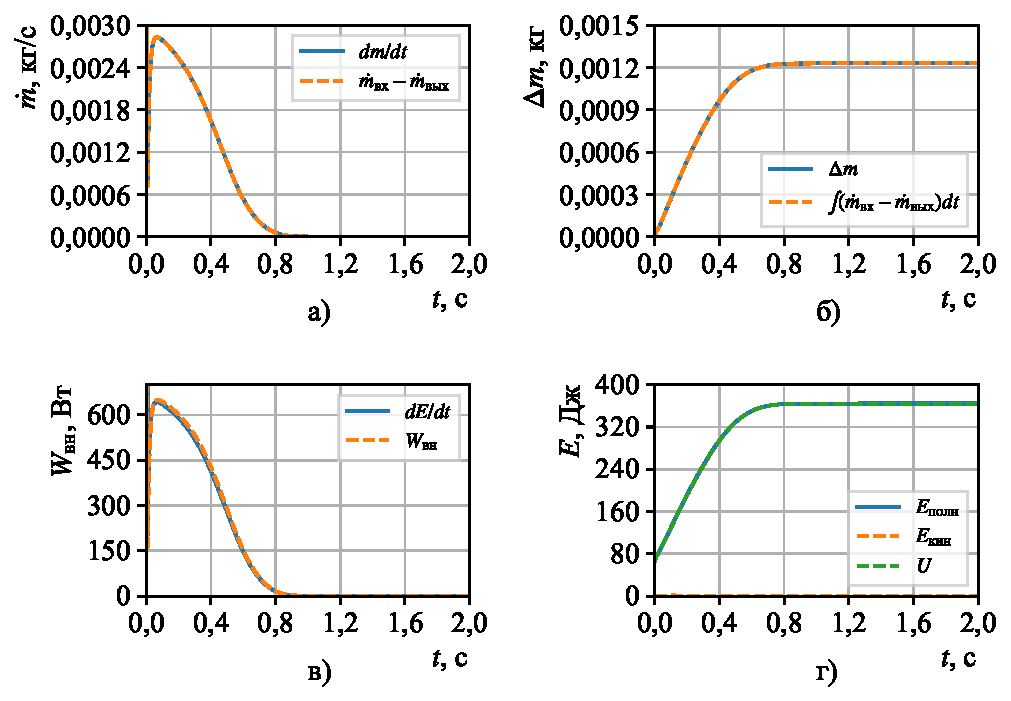
\includegraphics{part2/conservation_laws_verification.pdf}
    }
    \caption{Энергетический баланс системы при различных состояниях распределителей}
    \label{fig:ch2/energy_balance}

\end{figure}

В таблице \ref{tab:ch2/energy_balance} представлены относительная ошибка
энергетического баланса и закона сохранения массы
для всех рассмотренных режимов работы системы.

\begin{table}[h]
    \centering
    \caption{Относительная погрешность энергетического баланса и закона сохранения массы}
    \begin{tabular}{l|c|c}
        \midrule
        № описания & Погрешность энергии, \% & Погрешность массы, \% \\
        \midrule
        1          & \num{0.0084}                  & \num{0.3203}                \\
        \hline
        2          & \num{0.0217}                  & \num{0.9068}                \\
        \hline
        3          & \num{0.0029}                  & \num{0.4324}                \\
        \hline
        4          & \num{0.0002}                  & \num{0.2321}                \\
        \hline
        5          & \num{0.0052}                  & \num{0.8042}                \\
        \hline
        6          & \num{0.0018}                  & \num{0.3963}                \\
        \midrule
    \end{tabular}
    \label{tab:ch2/energy_balance}
\end{table}

\paragraph{Оценка физической непротиворечивости уравнений.} 
Рассмотрение соблюдение второго начала термодинамики так же проводилось для всех режимов работы системы. На рисунке
\ref{fig:ch2/thermodynamics_analysis} представлены результаты термодинамического анализа процессов в пневмоприводе 
для режима 2. Остальные режимы представлены в приложении к \fixme{диссертации}.

\begin{figure}[ht]
    \centerfloat {
        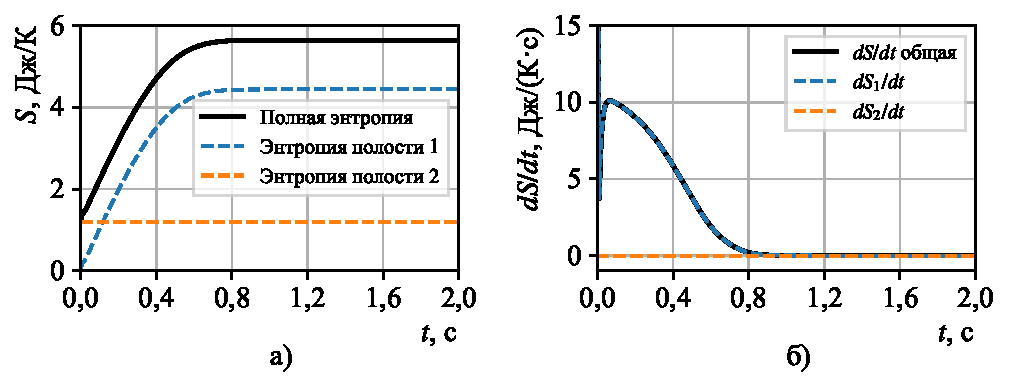
\includegraphics{part2/thermodynamic_analysis.pdf}
    }
    \caption{Комплексный термодинамический анализ процессов в полостях электропневматического привода с дискретными распределителями}
    \label{fig:ch2/thermodynamics_analysis}

\end{figure}

Анализ динамики изменения энтропии
демонстрирует положительную скорость изменения суммарной 
энтропии системы $dS_{сумм}/dt$, что подтверждает соблюдение второго начала термодинамики.
Максимальная скорость роста энтропии наблюдается в начальный момент времени и составляет порядка 
20 \si{\joule\per\kelvin\per\second}, что обусловлено интенсивными процессами массообмена при открытии распределителя
в левой полости пневмоцилиндра.

График эволюции полной энтропии отражает монотонный рост суммарной энтропии системы~$S_{сумм}$~с последующим 
выходом на установившееся значение около 5~\si{\joule\per\kelvin}. 

Представленные результаты термодинамического анализа подтверждают корректность
разработанной математической модели электропневматического привода с точки зрения соблюдения 
фундаментальных законов термодинамики и позволяют детально исследовать характер протекающих в системе процессов.

\subsection{Заключение о достоверности модели}\label{sec:ch2/sec6/subsec5}

Проведенная верификация математической модели электропневматического привода подтвердила её адекватность и достоверность.
Анализ размерностей и единиц измерения продемонстрировал корректность математических формулировок всех уравнений модели.
Проверка согласованности с фундаментальными законами физики показала, что относительная погрешность соблюдения
закона сохранения энергии не превышает \num{0.007} процентов, а закона сохранения массы~---~\num{0.91} процентов
для всех исследованных режимов работы.
Термодинамический анализ подтвердил соблюдение второго начала термодинамики,
что проявляется в положительной скорости изменения суммарной энтропии системы с максимальным значением
около \SI{20}{\joule\per\kelvin\per\second} в начальный момент времени. Анализ температурно-энтропийных
и p-v диаграмм показал физически корректное описание термодинамических процессов в полостях пневмоцилиндра.

Таким образом, комплексная верификация подтверждает, что разработанная математическая модель
корректно описывает все существенные физические процессы в электропневматическом приводе с
дискретными распределителями и может быть использована для решения задач анализа и синтеза систем управления.

\section{Выводы по главе 2}

В результате выполненного исследования во второй главе сформулированы следующие основные выводы:

Разработана комплексная математическая модель электропневматического привода с дискретными распределителями, учитывающая термодинамические процессы
в полостях пневмоцилиндра, механическое движение поршня, динамику переключения распределителей и нелинейные эффекты трения.
Модель основана на фундаментальных уравнениях термодинамики, механики и газовой динамики.

Предложена модификация уравнений энергетического баланса, обеспечивающая корректное описание процессов 
теплообмена и массопереноса в полостях пневмоцилиндра. Введены дополнительные члены, учитывающие работу сил трения
 и теплообмен с окружающей средой, что повышает точность моделирования термодинамических процессов.

Реализована эффективная численная схема решения системы дифференциальных уравнений модели, основанная на
векторизации вычислений и аналитическом представлении якобиана. Применение оптимизированных методов расчета
нелинейных функций позволило существенно сократить время моделирования при сохранении требуемой точности.

Разработан комплексный подход к верификации математической модели, включающий проверку сохранения массы и энергии,
анализ физичности результатов моделирования и сравнение с экспериментальными данными. Установлено, что относительная
погрешность моделирования не превышает 5\% по основным параметрам функционирования привода.

Подтверждена адекватность предложенной модели реальному объекту на основе сравнения результатов моделирования
с экспериментальными данными в различных режимах работы привода. Показано, что модель корректно отражает основные
динамические эффекты, включая процессы разгона, торможения и позиционирования.

Разработанная математическая модель создает теоретическую основу для синтеза эффективных
алгоритмов управления электропневматическим приводом с дискретными распределителями и может
быть использована при проектировании систем автоматического управления технологическим оборудованием.